\section{2b. Processor, Inputs and Outputs}

\begin{parag}{The cpu}
    As said before, the cpu is a very \important{sequential} component (but from now on we may omit the \important{clock} in diagrams). Therefore here we only have one data bus for read and write in our processor. The question we have is how can we handle input and ouput with only one data bus?
\end{parag}
\begin{parag}{Memory}
    At the moment we only need to speak about memory, connecting the cpu with the memory is pretty \textit{easy} as seen before
	\begin{center}
	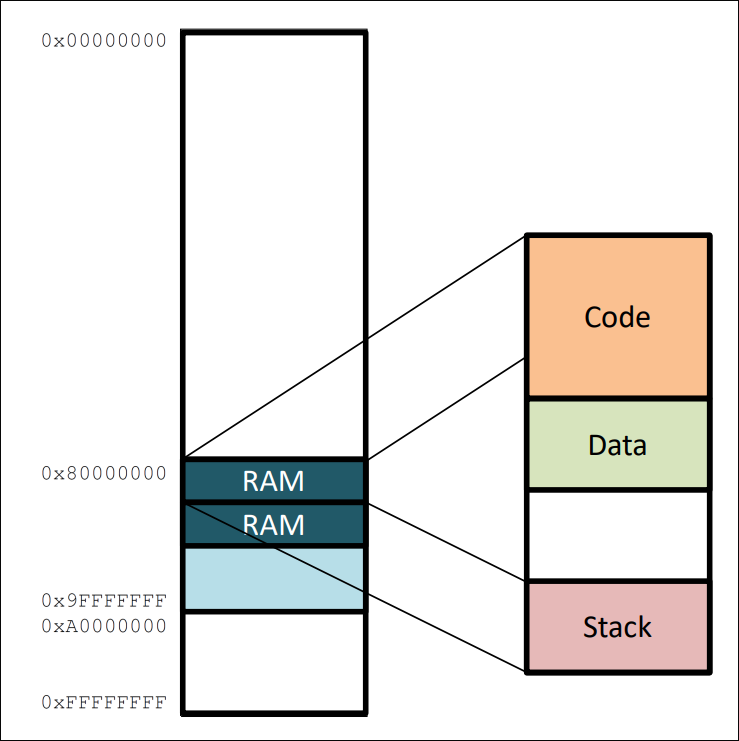
\includegraphics[scale=0.3]{screenshots/2025-10-22_3.png}
	\end{center}
	We assume that the ram begins at the  address \texttt{0x80000000} and then add what is needed to be added:
	\begin{center}
	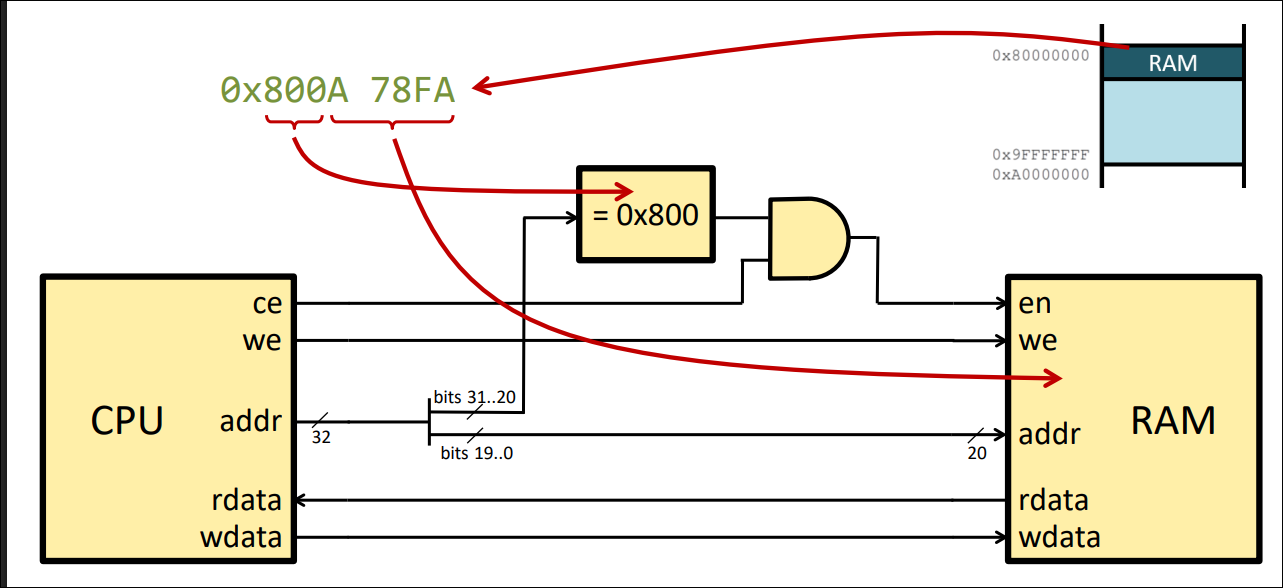
\includegraphics[scale=0.2]{screenshots/2025-10-22_4.png}
	\end{center}
\end{parag}
\begin{parag}{Input and Outputs device}
    As said before we only have 5 classic components of a computer, from where can we get our I/Os then? the way of doing this, is to use memory, we say that the device are just some value in memory with a certain address. However for this we have somme issue:\\
	Some device are way faster than other for instance here's a table of some example.
\end{parag}
	\begin{table}[h!]
\centering
\begin{tabular}{|l|l|l|}
\hline
\textbf{Type} & \textbf{Peripheral} & \textbf{Data Rate} \\ \hline
\multirow{2}{*}{Human Interaction} & Keyboard & $\sim$kbps \\
 & Mouse & $\sim$kbps \\ \hline
\multirow{3}{*}{Generic} & Serial Port (RS-232) & 115.2 kbps (max) \\
 & Parallel Port (LPT) & 150 kbps \\
 & USB 4.0 & 20--40 Gbps \\ \hline
\multirow{2}{*}{Generic (Wireless)} & Bluetooth 5.0 & 2 Mbps \\
 & PCIe 4.0 & 16 Gbps per lane \\ \hline
\multirow{2}{*}{Storage} & SATA III (HDD/SSD) & 6.0 Gbps \\
 & NVMe (PCIe 4.0) & 64 Gbps (4-lane) \\ \hline
\multirow{3}{*}{Networking} & Ethernet (10BASE-T) & 10 Mbps \\
 & 10 Gigabit Ethernet (10GBASE-T) & 10 Gbps \\
 & Wi-Fi 6 (802.11ax) & Up to 9.6 Gbps \\ \hline
\multirow{2}{*}{Displays} & VGA (analog video) & 0.6--1.5 Gbps (approx.) \\
 & HDMI 2.1 & 48 Gbps \\ \hline
\multirow{3}{*}{Optical Discs} & CD-ROM & 150 KB/s (1x) -- 7.68 MB/s (52x) \\
 & DVD-ROM & 1.32 MB/s (1x) -- 21.1 MB/s (16x) \\
 & Blu-ray & 4.5 MB/s (1x) -- 54 MB/s (12x) \\ \hline
\end{tabular}
\caption{Approximate data rates for common peripheral interfaces.}
\end{table}
\begin{parag}{Accessing I/Os: Port Mapped I/O (PMIO)}
    The way for this is to create a \important{new interface} similar to the memory one.\\
	We add the to CPU the port \texttt{ctrl-IO} and \texttt{port} Which serves as circuit enable and output enable. (this way, we'll know when accessing memory or I/O).\\
	It implies that we can create new instructions (e.g., \important{x86} but seldom used):
	\begin{itemize}
	    \item \texttt{IN register, port}
		\item \texttt{OUT port, register}
		\item For instance \texttt{IN al, Keyboard}
	\end{itemize}
\end{parag}
\begin{parag}{Accessing I/Os: Memory Mapped I/O (MMIO)}
    In this way, we don't make any difference between memory and I/Os.
	\begin{center}
	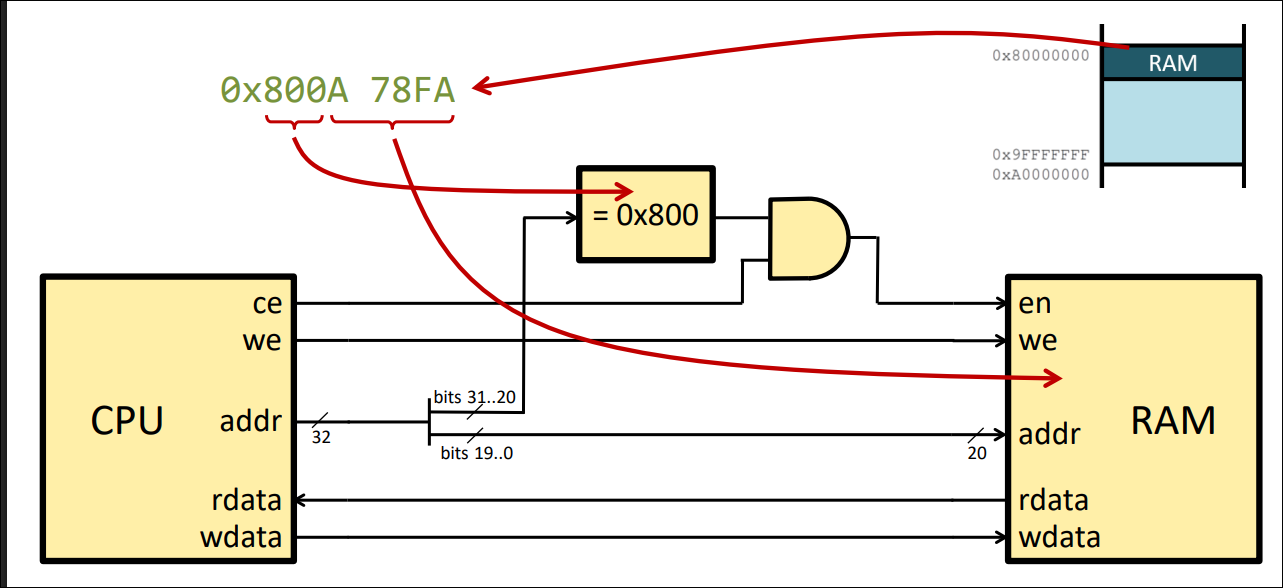
\includegraphics[scale=0.2]{screenshots/2025-10-22_4.png}
	\end{center}
	This means that there are no special hardware needed in the cpu $\implies$ no special instructions needed. For intsance in our example if we wanted to write a new value in the led:
	\begin{lstlistings}[language={[RISC-V]Assembler}]
lui t0, 0x10000 # pointer to I/Os
sw t1, 0(t0) # write LEDs
	\end{lstlistings}
	This means that we have a big data bus and depending on the value \important{the bus} choose between the Memory and the I/O 
	\begin{center}
	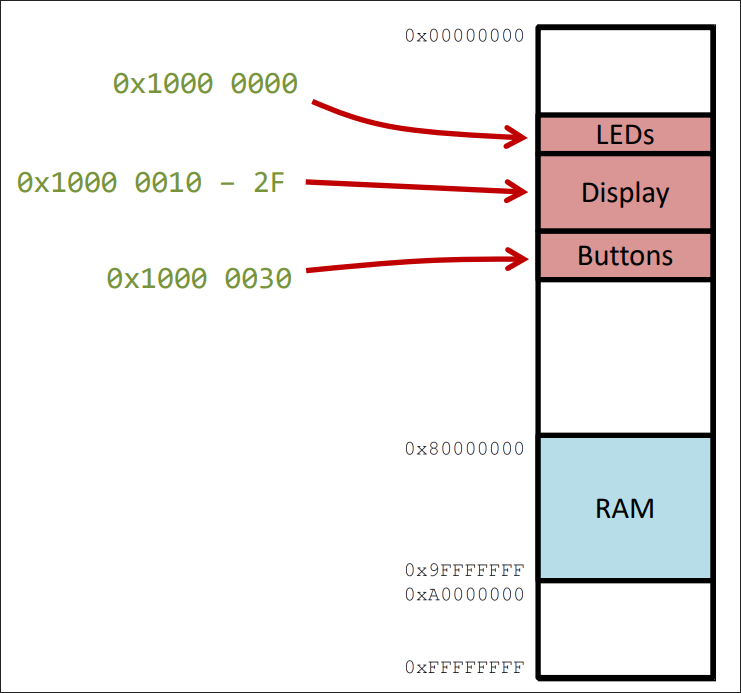
\includegraphics[scale=0.2]{screenshots/2025-10-22_5.png}
	\end{center}
\end{parag}
\begin{parag}{Example: A/D converter}
    An A/D converter is a device that \important{converts an analog signal into a digital signal}. What we need is:
	\begin{enumerate}
	    \item \important{Start} (\texttt{START}): input; when active begins a new conversion
	    \item \important{Data Valid} (\texttt{/DV}): outputl when active, D7-D0 are valid
	    \item \important{Data} (D7-D0): output; last conversion result
	\end{enumerate}
	\begin{center}
	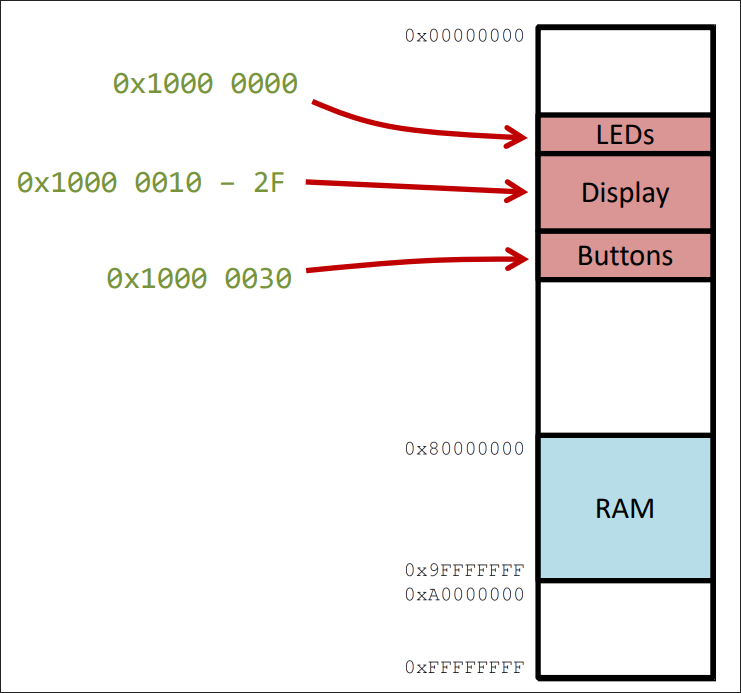
\includegraphics[scale=0.2]{screenshots/2025-10-22_5.png}
	\end{center}
	
\end{parag}


\begin{parag}{Example: Simple bus interface}
    Suppose that a 8-bit processor has the following signals:
	\begin{itemize}
	    \item \important{Address} (A23-A0): output; address bus
		\item \important{Data} (D7-D0): inputl data bus 
		\item \important{Adress Strobe} (/AS) output, signals the presence of a valid address on the Address bus during a memory access cycle
		\item \important{Read/Write} (R/W): output; signal the direction of the data flow
		\item \important{Data Acknowledge} (/DTACK): input; must be activated at the end of a memory access, when the written data have been latched or the read data are ready 
	\end{itemize}
	This is similar but not identical to the MC6800
	\begin{framedremark}
	ChatGPT on the mc68000:\\
	The MC68000 (also called the Motorola 68000) is a 16/32-bit microprocessor that was very popular in the late 1970s and 1980s. It was used in systems like the original Apple Macintosh, Amiga computers, and early Sun workstations. In your example, it’s mentioned as a reference because the bus signals are similar to those on the 68000, but not exactly the same.\\
	\textbf{in short}: the MC68000 is just a classic CPU used as a reference for teaching how these buses work.
	\end{framedremark}
	
\end{parag}
The goal now for us is to create a circuit that is able to connect the A/D converter to the processor (the MC68000). For this we will use a \important{memory mapped interface}. \\
We want that:
\begin{itemize}
    \item \important{any access} (\texttt{R} or \texttt{W}) to address \texttt{0xFFFF0} starts a \important{new conversion}
    \item The \important{data valid} signal can be read by the processor at address \texttt{0xFFFF4} (bit 0)
    \item The \important{result of the conversion} can be read by the processor at address \texttt{0xFFFF8}
\end{itemize}
Here's a little diagram of the state
\begin{center}
	    
	
\begin{tikzpicture}[
    state/.style=
	{circle, mininum size=0cm, draw, align=center, ->, >, >=stealth', auto, semithick },
    >=Stealth
]

% Nodes
\node[state]  at (0, 0)(execute) {Start memory\\ access};
\node[state] at (-4, 0)(left){};
\node[state] at (4, 0)(right){};

% Arrows
% Loop back arrows
\draw (execute) edge[loop above] node {\texttt{/DTACK} == 1} (exectute);
\draw[->] (execute.west) edge[bend left] node {\texttt{/DTACK} == 0} (left);

\draw[->] (right) edge[bend left] node {\texttt{mem\_type} == 1} (execute.east);
\end{tikzpicture}

\end{center}

To be able to construc the circuit we have to be careful about the timing diagram here; the fact that the ADDR and the /AS responds only at the clock edge gives us the information that we will need a \textit{register} which stores the DTACK signal and then output the As and ADDR signal after. This big register here is the \important{processor}.
\begin{center}
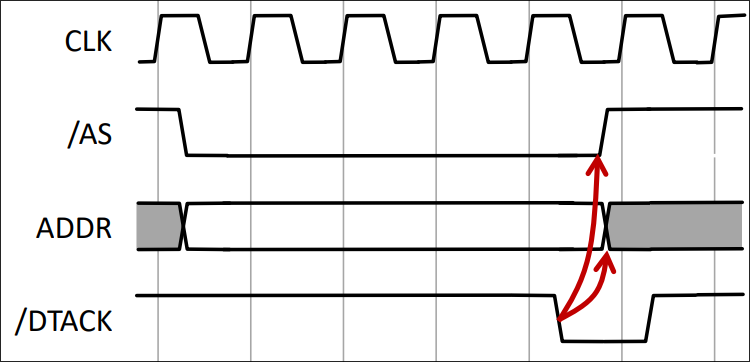
\includegraphics[scale=0.2]{screenshots/2025-10-22_8.png}
\end{center}
\begin{center}
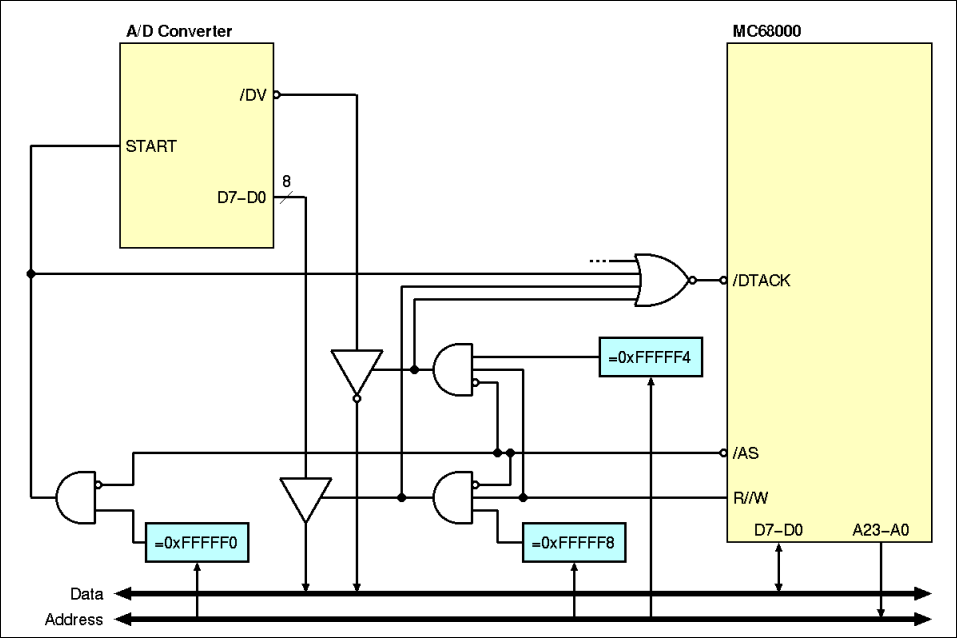
\includegraphics[scale=0.2]{screenshots/2025-10-22_9.png}
\end{center}
\begin{framedremark}
Here we can see that we have two tri-state buffer, but why? It is pretty rare for us to see tri-state buffer so why are they usefule here?\\
The answer is that they serve as a multiplexer between the DV and D7-D0, you can look at it and if you thing about it the two tri state buffer really serve as a \textit{decentralized} multiplexer.
\end{framedremark}

\begin{parag}{A/D converter: software}
    Let us now loot at it as a software person which is pretty easy because of the MMIO:
	\begin{lstlistings}[language={[RISC-V]Assembler}]
read\_adc: 
	lui t1, 0xfff 
	addi t1, t1, 0xff0 #t1 = 0xfffff0
	sw zero, 0(t1) # start conversion 
poll:
	lw t0, 4(t1) # t0 = DV signal 
	beqz t0, poll  # wait until done

end:
	lw a0, 8(t1) # a0 = A/D output 
	ret
	\end{lstlistings}
\end{parag}




\begin{parag}{Programmed I/Os}
    \important{Many peripherals} are more developped programmable systems and have a set of registers which the processor reads and writes (a) to \important{send} and \important{receive data} and (b) to \important{issue commands} and \important{read the status}.
	\begin{center}
	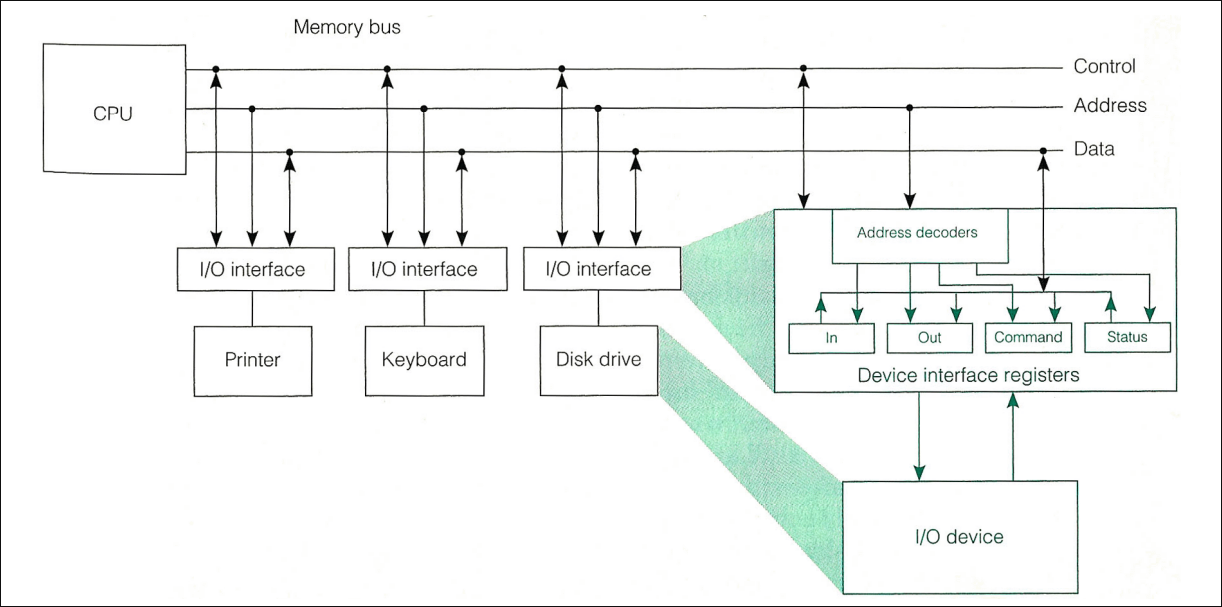
\includegraphics[scale=0.2]{screenshots/2025-10-22_10.png}
	\end{center}
\end{parag}

\subsection{A Classic UART}

\begin{parag}{Definition}
    A \important{UART} means: Universal Asynchronous Receiver-Transmitter\\
	This is one of the \important{simplest and most common communication} peripherals, it is typically used today to connect terminals to embedded devices. Our UART has a \important{simple programmed I/O interface} with four registers:
	\begin{itemize}
	    \item A \important{control register} for the processor to configure the UART 
			\begin{itemize}
				\item Bit 7 must be set to 1 for the UART to be enabled
				\item Bits 2..0 configure the communication speed (e.g., 0b001 for 9600 baud)
			\end{itemize}
		\item a \important{status register} for the processor to check the status of the UART
			\begin{itemize}
				\item Bit 1 is 1 if there are data available
				\item Bit 0 is 1 if the UART is ready to send data
			\end{itemize}
			\item A \important{data input} register where the received  data are available to the processor
			\item A \important{data output} register where the processor places data to send
	\end{itemize}
\end{parag}
\begin{lstlisting}[language={[RISC-V]Assembler}]
UART\_CTRL\_ADDR = 0x10000000 # UART status register address
UART\_ENABLE\_BIT = 0x80 # Enable bit (bit 7)
UART\_SPEED\_9600 = 0x01 # Speed setting for 9600 baud (4 bits, [3:0])
UART\_STATUS\_ADDR = 0x10000004 # UART status register address
TX\_READY\_BIT = 0x01 # Transmitter ready bit (bit 0)
UART\_DATAIN\_ADDR = 0x10000008 # UART data input (receive) register address
UART\_DATAOUT\_ADDR = 0x1000000C # UART data output (send) register address
send\_string:
	li t0, UART\_CTRL\_ADDR # Get UART control address
	li t1, UART\_STATUS\_ADDR # Get UART status address
	li t2, UART\_DATAOUT\_ADDR # Get UART data address
	li t3, UART\_ENABLE\_BIT # Get enable bit (0x80)
	li t4, UART\_SPEED\_9600 # Get speed setting (0x01)
	or t4, t3, t4 # Combine enable and speed bits
	sw t4, 0(t0) # Configure using the UART control register
next\_char:
	lb t5, 0(a0) # Load first byte of the string
	beqz t5, finish # If byte is zero (null terminator), finish
check\_tx\_ready:
	lw t6, 0(t1) # Load UART status register
	andi t6, t6, TX\_READY\_BIT # Check if TX\_READY\_BIT is set
	beqz t6, check\_tx\_ready # If not ready, loop back and check again
	sw t5, 0(t2) # Store the character in UART data register
	addi a0, a0, 1 # Increment string pointer (move to next char)
	j next_char # Jump back to send the next character
finish:
	ret # Return when the string is done
\end{lstlisting}
	
	

\begin{parag}{I/O polling}
    Everything we did is nice however there is still some issue: \important{polling}\\ The issue with polling is that the cpu is \textit{waiting} until the polling is done which is slowing down the cpu (a lot). Moreover, how do we even know if a peripheral has data for us (key pressed, packet arrrived, etc.)? we are not able to polled everything. \\
	For something like a keyboard which would only need to check every ms (approximatively) it would be \textit{okay} however imagine a usb or an ethernet cable this is not managable.
	\begin{center}
	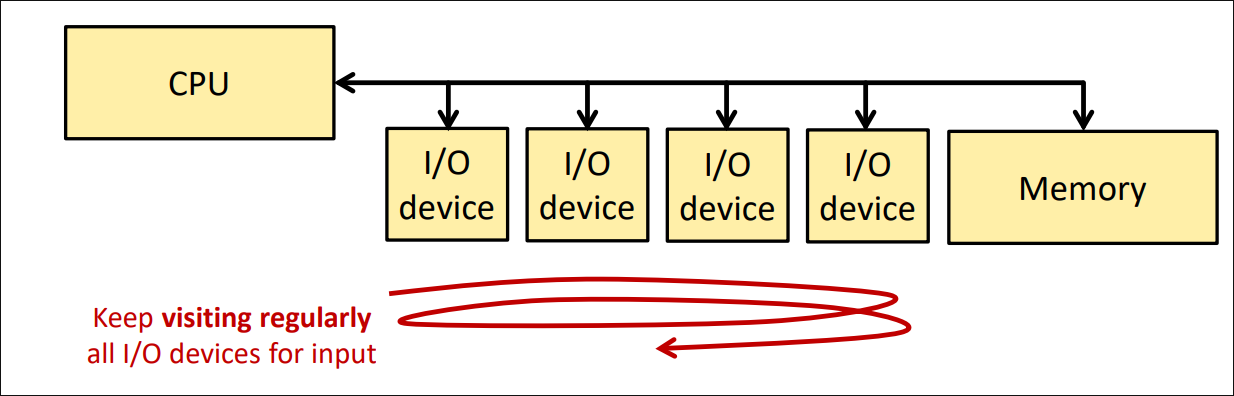
\includegraphics[scale=0.2]{screenshots/2025-10-22_11.png}
	\end{center}
\end{parag}


